\section{Software Project Management Plan}

\subsection{Project Planning}

We planned the work in eight four-week sprints (Table~\ref{tab:timeframe}). Sprint~1 covers requirements and design, Sprints~2--7 build the modules, and Sprint~8 is kept for integration, testing and the demonstration. A task is done when its code and tests pass and its part of this report is updated. The work is broken down in the Work Breakdown Structure (WBS) of Section~\ref{sec:wbs} \cite{wbs1}.

\subsubsection{Milestones Plan}
\label{sec:milestones}

Table~\ref{tab:milestones} lists the seven milestones of the plan. Each row gives the week in which the milestone falls due and the evidence that shows it was reached.

\begin{table}[!ht]
\centering
\caption{Project Milestones}
\label{tab:milestones}
{\small\renewcommand{\arraystretch}{1.1}
\begin{tabularx}{\textwidth}{c>{\raggedright\arraybackslash}X>{\centering\arraybackslash}p{1.4cm}>{\raggedright\arraybackslash}p{4.9cm}}
\hline\hline
\textbf{ID} & \textbf{Milestone} & \textbf{Week} & \textbf{Evidence of completion} \\
\hline
MS1 & FYP-I proposal submitted & Before 1 & Proposal, 24 Feb 2026 \\
MS2 & Requirements, product backlog and architecture agreed & 4 & Scope approved \\
MS3 & Login, device binding and roles working (M1, M7) & 8 & Module tests pass \\
MS4 & FYP-I review & 16 & FYP-I report submitted, 18 Jun 2026 \\
MS5 & Supervision, submission and evaluation working (M5, M6, M10, M11) & 24 & Module tests pass \\
MS6 & All twelve modules merged (M12 last) & 28 & Module tests pass (M2 and M4 tests finished in Sprint~8) \\
MS7 & Final test run and submission & 32 & Full test run, 26 Oct 2026 \\
\hline\hline
\end{tabularx}}
\end{table}

\subsubsection{Documentation Plan}

The report is kept in step with the code:
\begin{itemize}[nosep]
    \item The report is written in LaTeX, and the section a task changes is updated in that task.
    \item Diagrams are kept as text sources beside the report, so they are redrawn when the design changes.
    \item Each version of the report is recorded in the Revision History, and supervisor feedback goes into the next sprint's backlog.
\end{itemize}

\subsubsection{Resources Plan}
\label{sec:resources_plan}

Table~\ref{tab:resources} lists the resources the project uses, one row for each kind. The project has no budget, so every service is a free plan or is off by default.

\begin{table}[!ht]
\centering
\caption{Project Resources}
\label{tab:resources}
{\small\renewcommand{\arraystretch}{1.2}
\begin{tabularx}{\textwidth}{>{\raggedright\arraybackslash}p{2.2cm}>{\raggedright\arraybackslash}X}
\hline\hline
\textbf{Resource} & \textbf{Allocation} \\
\hline
People & Three members, each owning one area (Section~\ref{sec:managerial}); the supervisor reviews every sprint. \\
Hardware & Our own PCs for development and the automated tests; Windows lab PCs, with webcams where an exam needs one, for the manual lockdown and webcam checks. \\
Software & .NET~9 (server and desktop client), React (web panel), PostgreSQL, OpenCV with the YuNet and YOLOX-Nano models, Docker with a GCC compiler image, xUnit, Playwright, Git, and LaTeX with PlantUML for this report. \\
Services & Neon cloud PostgreSQL (free plan), an e-mail account for notifications, and an optional AI language-model service for theory marking that is off by default. \\
Budget & None: no paid service is used. \\
\hline\hline
\end{tabularx}}
\end{table}

\subsubsection{Quality Plan}

Quality is checked inside every sprint, not only at the end:
\begin{itemize}[nosep]
    \item Each module is tested in its own sprint with server, web and desktop tests, and the full test suite is rerun after each group of fixes.
    \item Checks that need a real lab PC are kept on a manual lab checklist (Chapter~\ref{chap:testing}).
    \item AI output is only a suggestion: the teacher reviews and can change every mark, and no violation leads to an automatic penalty.
    \item The supervisor reviews each increment at the end of the sprint.
\end{itemize}

\subsection{Project Scheduling}
\label{sec:scheduling}

\subsubsection{Gantt Chart}

Table~\ref{tab:cpm} lists the nine project activities with their modules, their length in weeks and the activities each must wait for. The Gantt chart and the critical path network are both drawn from this table.

\begin{table}[!htbp]
\centering
\caption{Project Activities, Durations and Dependencies}
\label{tab:cpm}
\renewcommand{\arraystretch}{1.2}
\begin{tabular}{c>{\raggedright\arraybackslash}p{7.2cm}lcc}
\hline\hline
\textbf{ID} & \textbf{Activity} & \textbf{Modules} & \textbf{Weeks} & \textbf{Depends on} \\
\hline
A & Requirements, backlog and architecture & -- & 4 & -- \\
B & Authentication and device binding & M1 & 4 & A \\
C & User and role management & M7 & 2 & A \\
D & Exam creation and eligibility & M8, M9 & 4 & B, C \\
E & Readiness check, student dashboard and lockdown & M2--M4 & 4 & D \\
F & Monitoring client and live proctoring dashboard & M5, M10 & 4 & E \\
G & Submission, backup and AI-assisted evaluation & M6, M11 & 4 & F \\
H & Audit log, analytics and reports & M12 & 4 & G \\
I & Integration, system testing, documentation and demo & All & 4 & H \\
\hline\hline
\end{tabular}
\end{table}

Figure~\ref{fig:ganttchart} places the activities of Table~\ref{tab:cpm} on Weeks 1--32 \cite{gantt1}. Red bars lie on the critical path, and the diamonds mark the FYP-I review and the final submission.

\begin{figure}[!htbp]
\centering
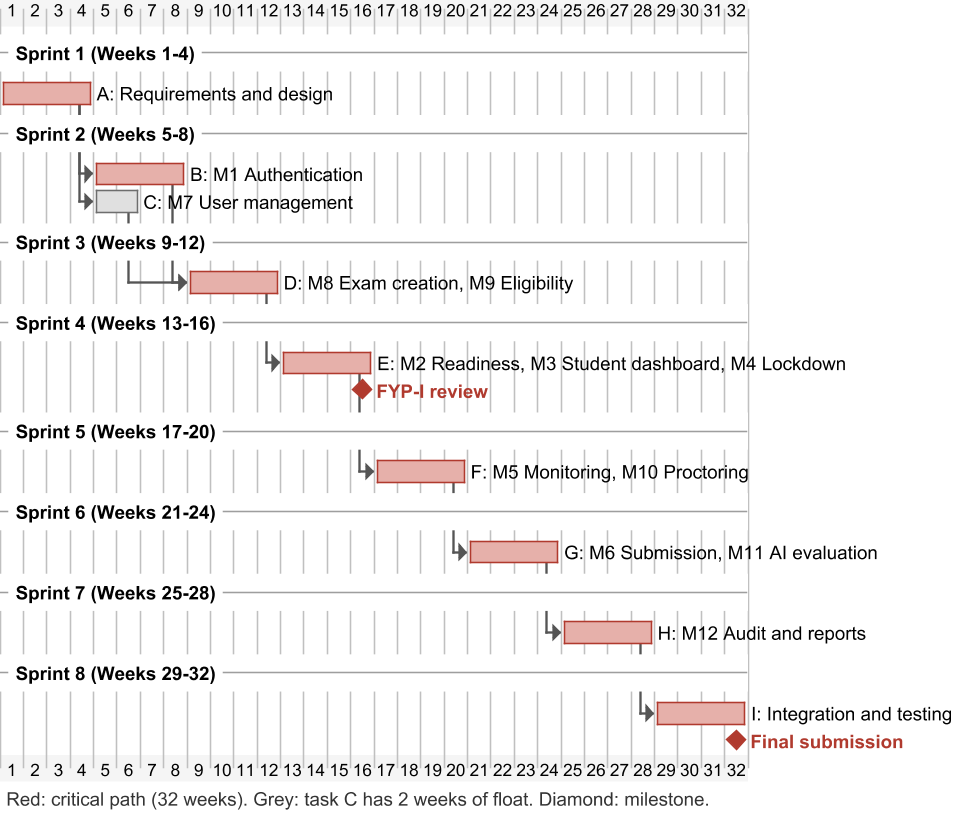
\includegraphics[width=\linewidth,height=0.8\textheight,keepaspectratio]{Figures/gantt_chart.png}
\caption{Project Gantt Chart (Baseline Plan, Eight Sprints)}
\label{fig:ganttchart}
\end{figure}

\DiagramBarrier
\subsubsection{Work Breakdown Structure}
\label{sec:wbs}

Figure~\ref{fig:wbs} splits the project into four main work packages \cite{wbs1}. Under Module Development, each module is one work package that includes its own tests.

\begin{figure}[!htbp]
\centering
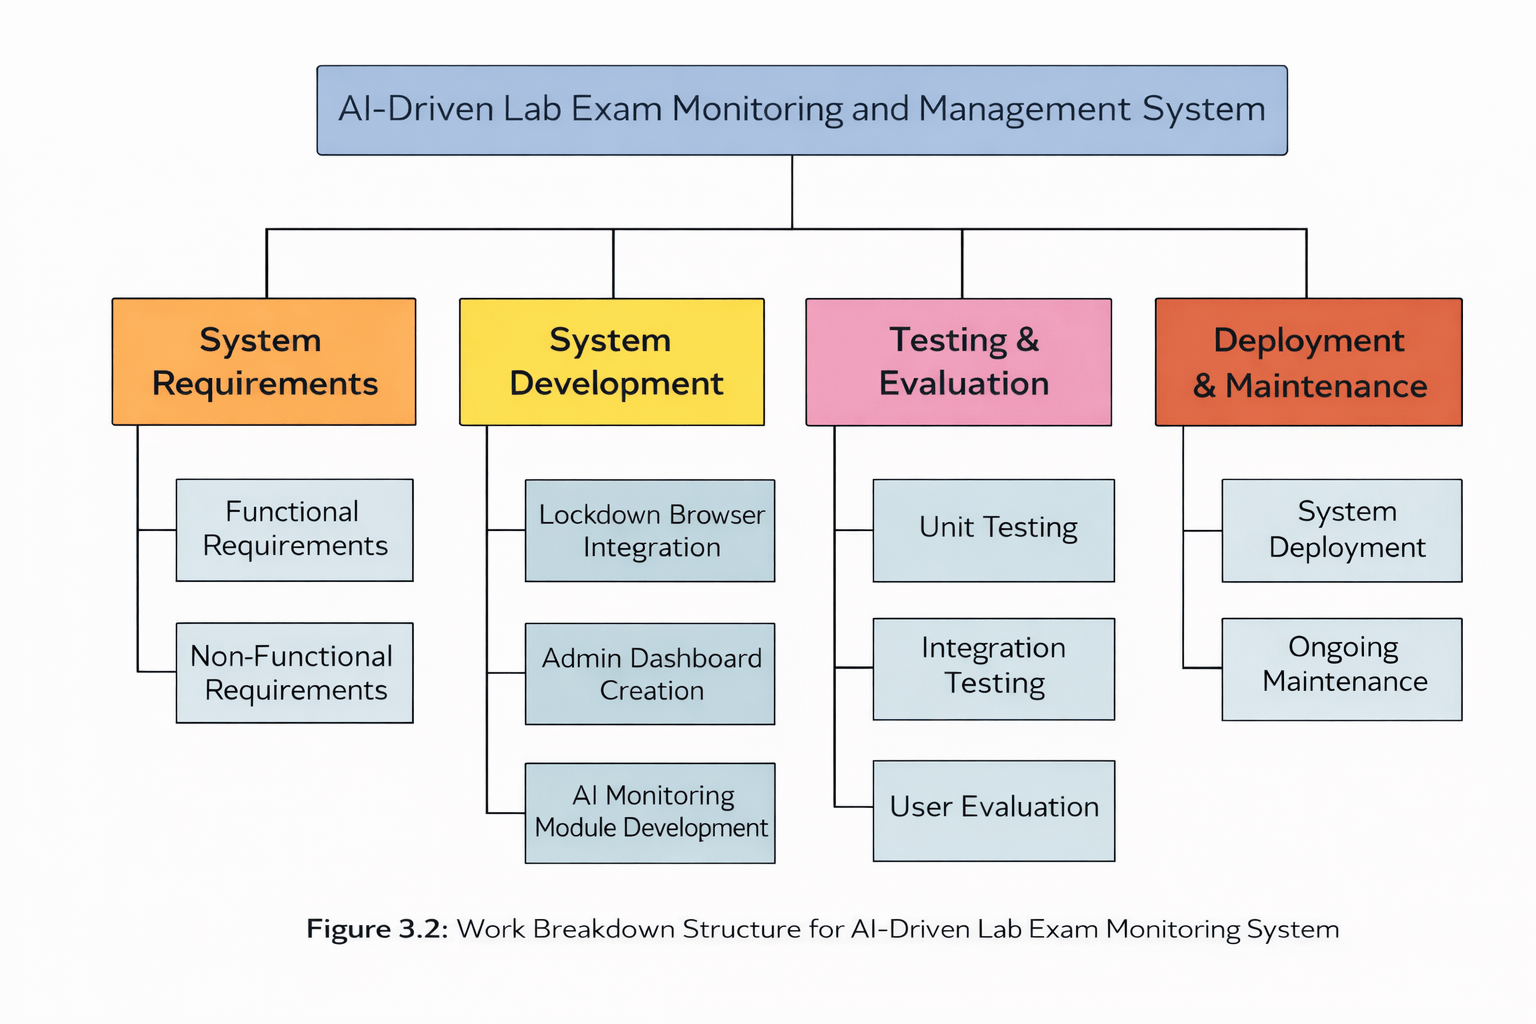
\includegraphics[width=\linewidth,height=0.8\textheight,keepaspectratio]{Figures/work_breakdown_structure.png}
\caption{Work Breakdown Structure}
\label{fig:wbs}
\end{figure}

\DiagramBarrier
\subsubsection{Critical Path Method}

The critical path is the longest chain of dependent activities; a delay on it delays the whole project \cite[Sec.~6.5.2.2]{pmbok6}. Since almost all our work lies on it, we tracked each sprint with a burn-down chart \cite{scrum1}; when less than 80\% of a sprint's story points were done at the review, backlog items were moved or cut.

Figure~\ref{fig:criticalpath} shows the network of Table~\ref{tab:cpm}. The path A--B--D--E--F--G--H--I takes 32 weeks; only C, which runs beside B, has two weeks of float.

\begin{figure}[!htbp]
\centering
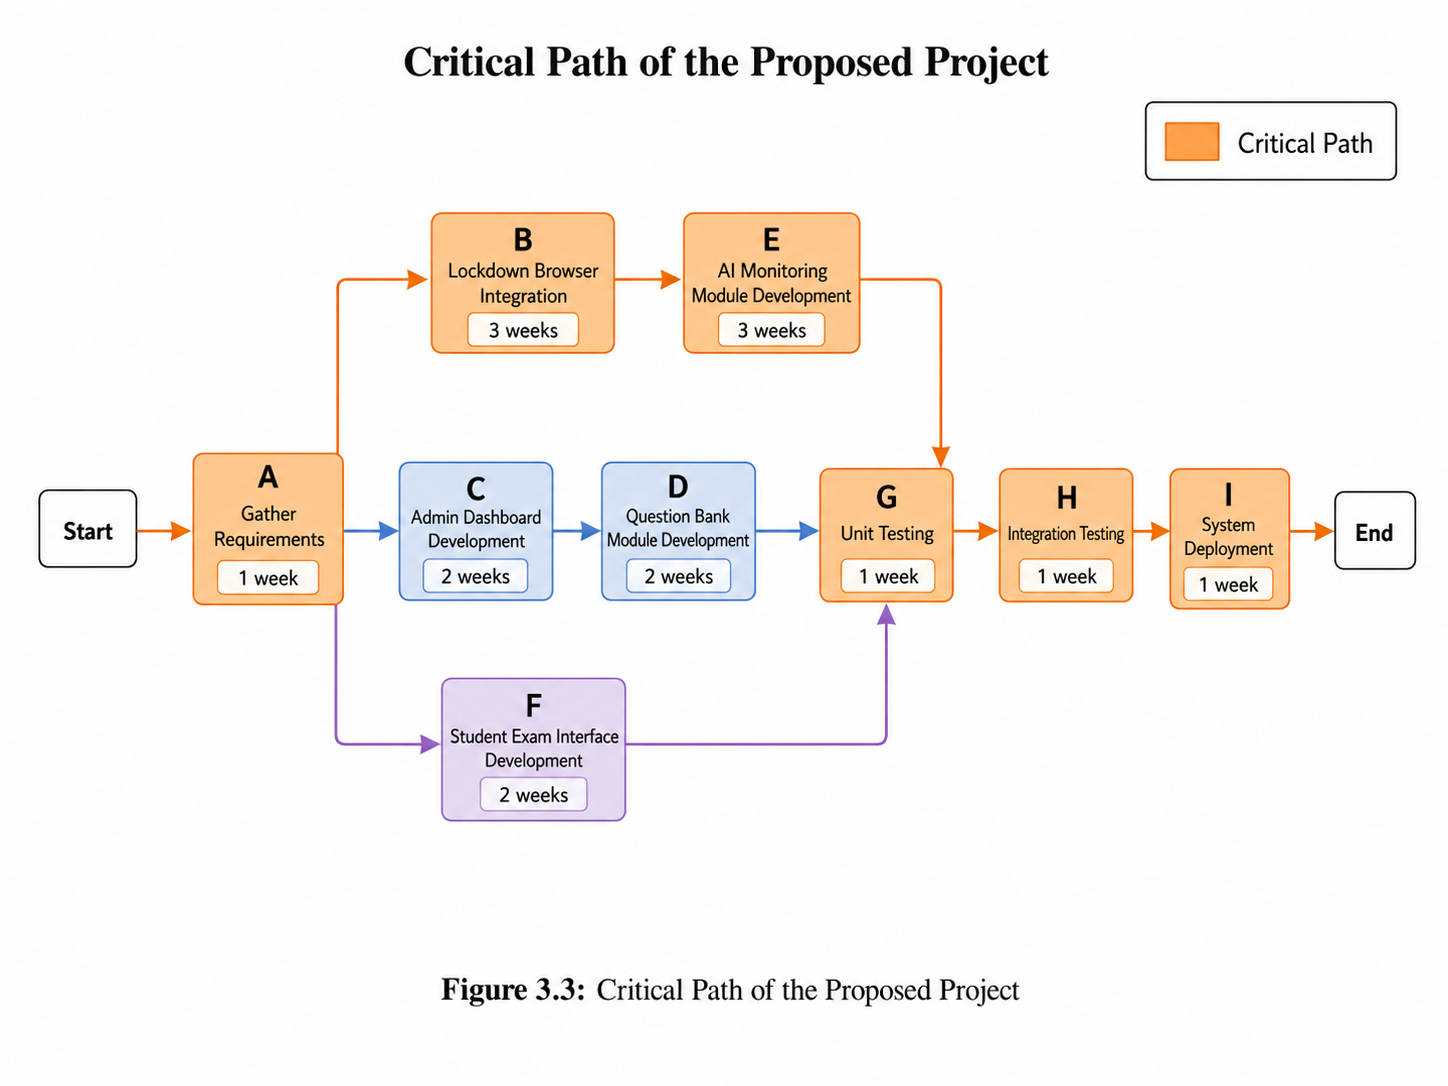
\includegraphics[width=\linewidth,height=0.8\textheight,keepaspectratio]{Figures/critical_path.png}
\caption{Critical Path Network}
\label{fig:criticalpath}
\end{figure}
\DiagramBarrier
